\chapter{Decision Trees}
\section{Introduction}
Decision trees are a popular method for various machine learning tasks. 
They are easy to understand and interpret, and the process of building a decision tree is intuitive.
\par
\noindent
{\large \textbf{Cats classification example:}}
\\
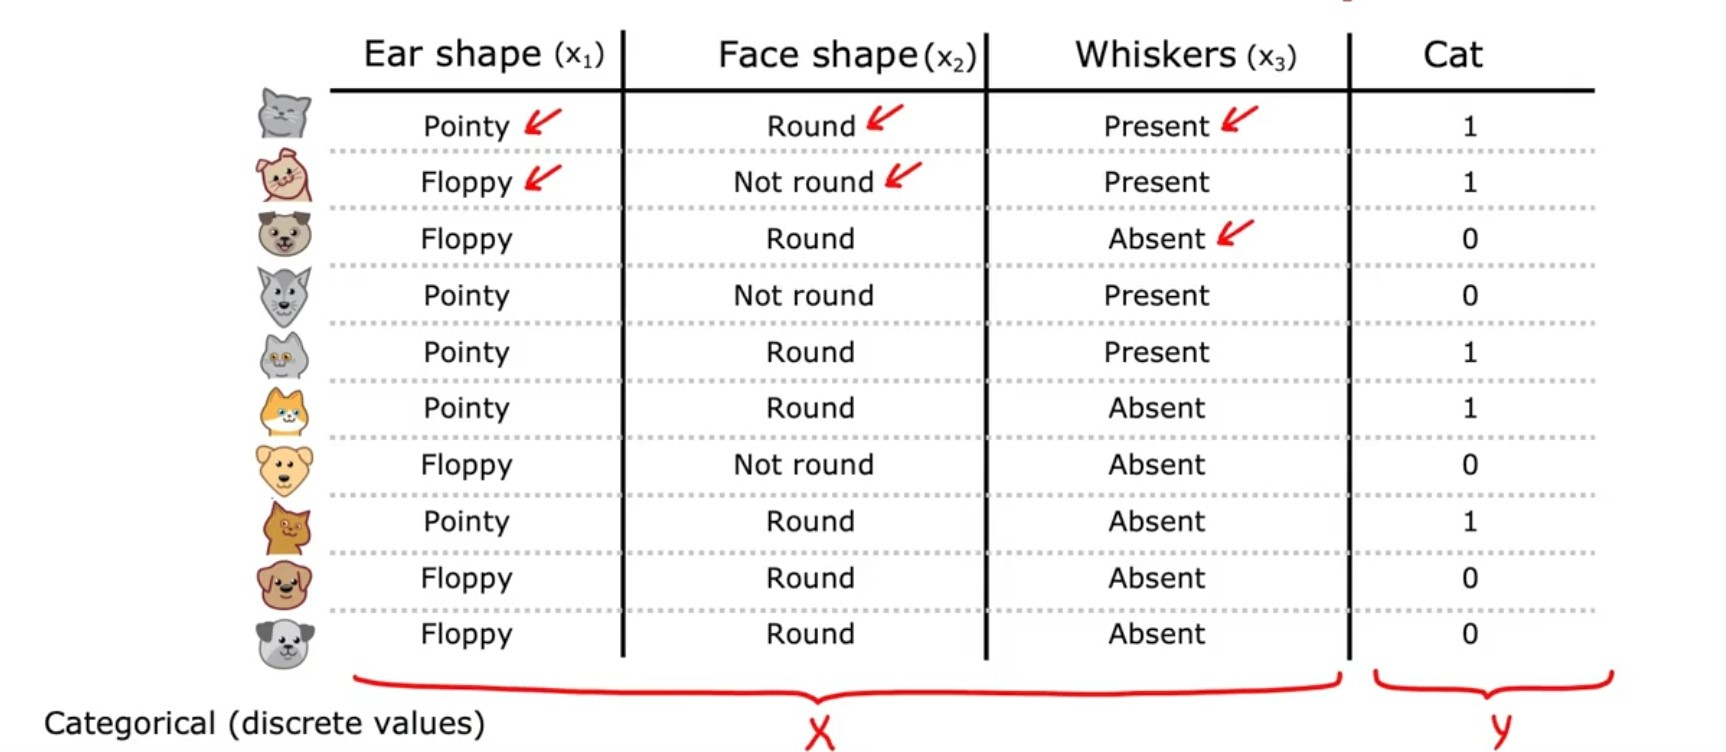
\includegraphics[width=\textwidth]{images/11.1}
\par
Decision tree model has the structure of a tree,
where each \textbf{decision node} represents a feature (attribute),  
and each \textbf{leaf node} represents the outcome.\\
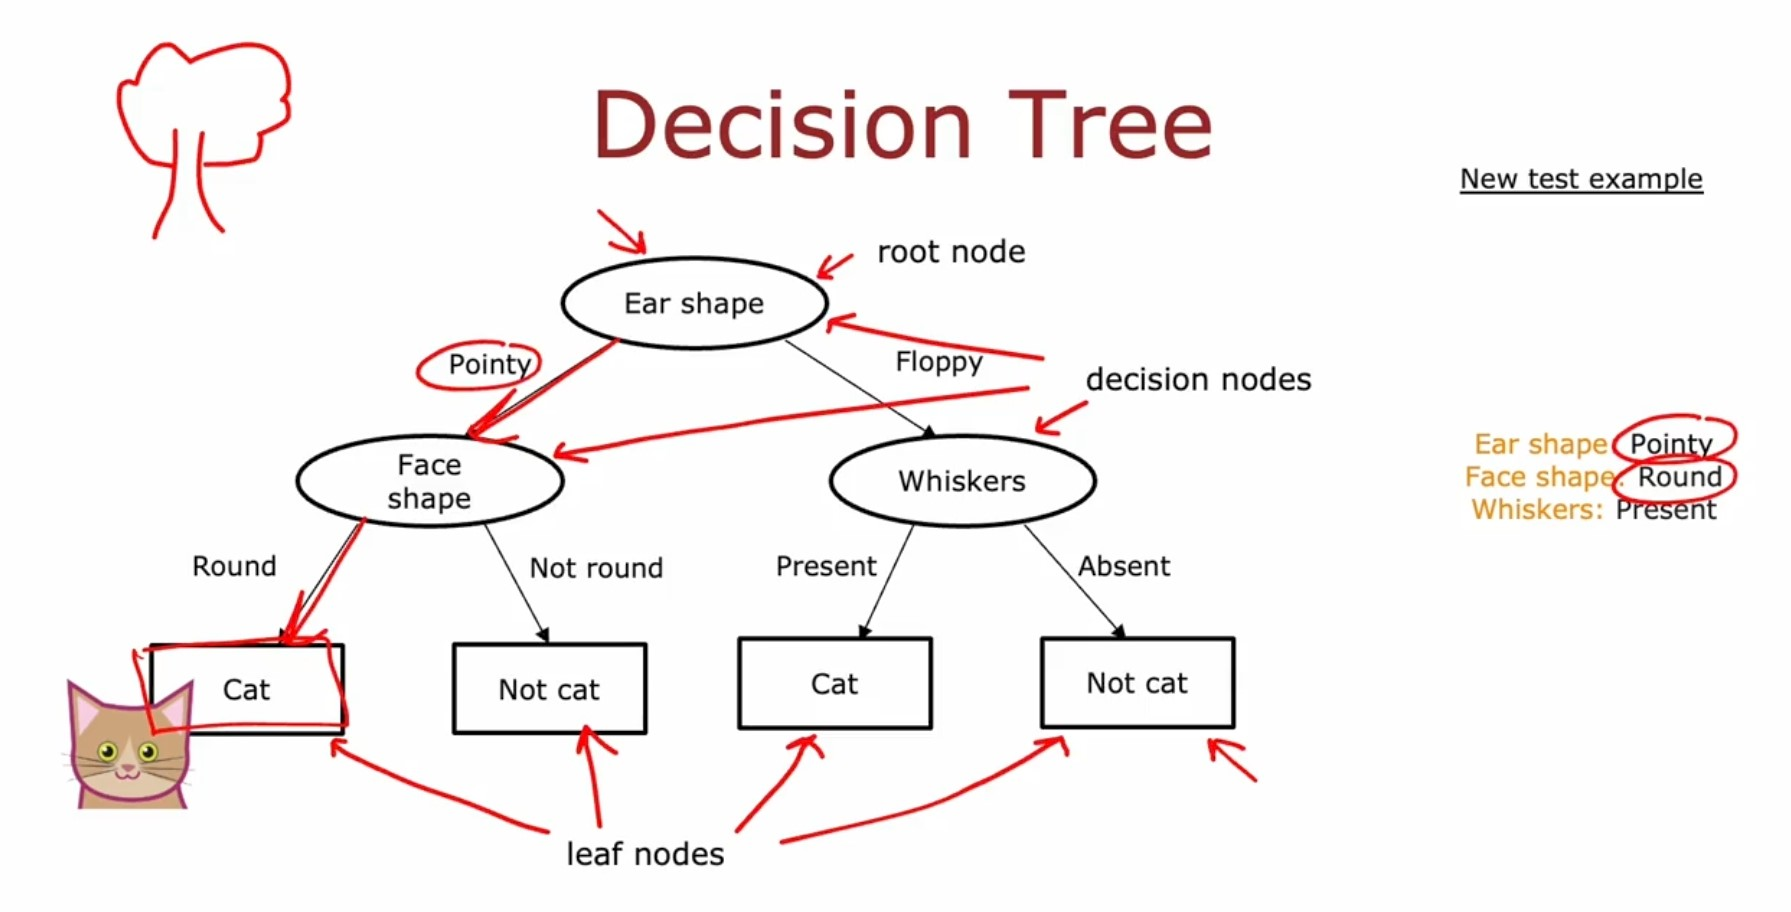
\includegraphics[width=\textwidth]{images/11.2}
\par
\subsection*{Learning process}
The algorithm's goal is to find the decision tree that best classifies the training data.
The learning process is divided into two steps:\par
\textbf{Decision 1:} How to choose what features to split on at each node?\\
maximize purity (minimize impurity) of the child nodes.\\
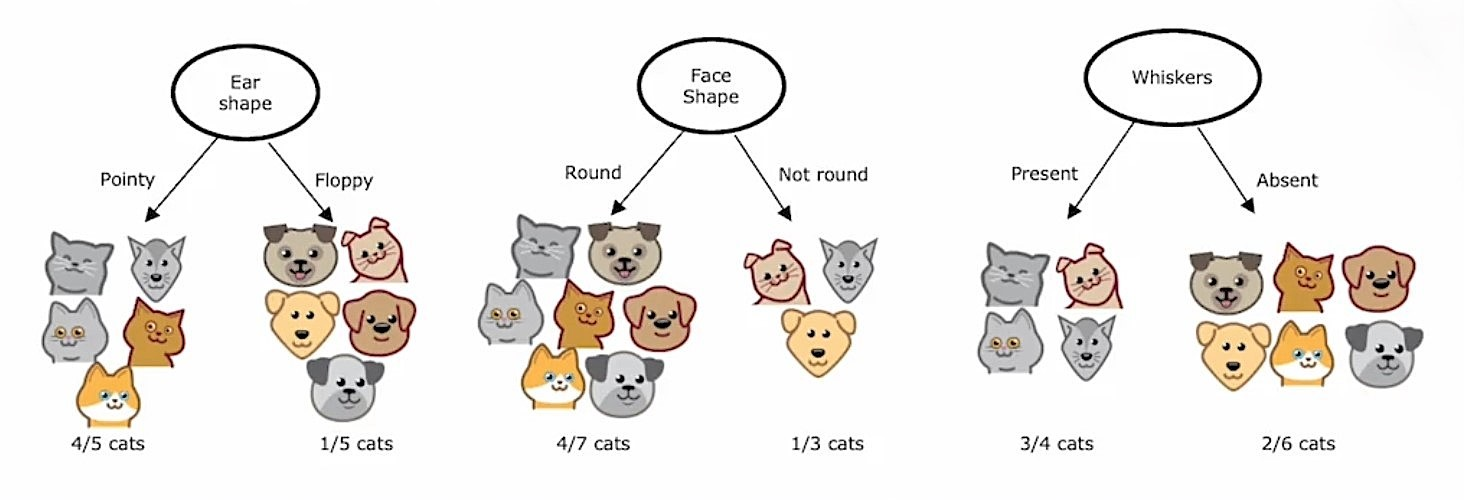
\includegraphics[width=\textwidth]{images/11.3}
\par
\textbf{Decision 2:} When to stop splitting?\\
\begin{itemize}
    \item When all data points in a node belong to the same class.
    \item When Exceeding a maximum depth.
    \item When impovements in purity are below a certain threshold.
    \item When the number of data points in a node is below a certain threshold.
\end{itemize}
\par
\includegraphics*[width=\textwidth]{images/11.4}
\par
The splitting method and stopping method have a lots of variance,
as the development of decision tree algorithm, many methods have been proposed.
\section{Decision tree learning}
\subsection*{Measuring purity}
\subsubsection*{Entropy}
Entropy is a measure of impurity.\\
\includegraphics*[width=\textwidth]{images/11.5}
\begin{thmbox}{Entropy}{e}
    \begin{align}
        H(x) &= -x\log_2(x) - (1-x)\log_2(1-x)\\
        &\text{note:} \quad 0\log_2(0) = 0 \nonumber
    \end{align}
\end{thmbox}
\subsection*{Information gain}
Choosing splits that maximize information gain.\\
\includegraphics*[width=\textwidth]{images/11.6}
\begin{thmbox}{Information gain}{i}
\begin{equation}
    IG = H(p_1^{\text{parent}}) - \left(w^{\text{left}}\cdot H\left(p_1^{\text{left}}\right) 
    + w^{\text{right}}\cdot H\left(p_1^{\text{right}}\right)\right)
\end{equation}
\end{thmbox}
\includegraphics*[width=\textwidth]{images/11.7}
\subsection*{Algorithm}
\begin{thmbox}{Decision tree algorithm}{d}
\begin{enumerate}
    \item \texttt{current node = root node}
    \item \texttt{While not stopping criteria:}
    \item[] \quad Calculate information gain for all features in current node
    \item[] \quad Pick the feature with the highest information gain
    \item[] \quad Split the node into child nodes according to the feature
    \item[] \quad \texttt{current node = next(current node)}
\end{enumerate}
\end{thmbox}
\par
This algorithm can be implemented recursively.
\begin{thmbox}{Decision tree algorithm pseudocode}{d}
\begin{minted}{python}
    def build_decision_tree(node, data):
        if stopping_criterion(node, data):
            return
        feature, threshold = find_best_split(data)
        left_data, right_data = split_data(data, feature, threshold)
        node.left = build_decision_tree(node.left, left_data)
        node.right = build_decision_tree(node.right, right_data)
        return node
\end{minted}
\end{thmbox}
\subsection*{One-hot encoding}
One-hot encoding is a method to convert categorical data into numerical data.
if a feature has $n$ categories, then it will be converted into $n$ binary features.\\
\includegraphics*[width=\textwidth]{images/11.8}
\subsection*{Splitting continuous variables}
Choose the best split point by calculating information gain for all possible split points.\\
\includegraphics*[width=\textwidth]{images/11.9}
\subsection*{Regression trees}
Regression trees are used for continuous target variables.\\
\includegraphics*[width=\textwidth]{images/11.11}
\par
Assume that we have built a decision tree model, 
and we want to predict the target value for a new data point.
The prediction is made by traversing the tree from the root node to a leaf node.
The target value of the leaf node (average of target values of the training data in that node) is the prediction.\\
\includegraphics*[width=\textwidth]{images/11.10}
\par
\noindent
{\large \textbf{Choosing a split:}}\par
\begin{itemize}
    \item Calculate the variance of the target values in the parent node.
    \item Calculate the variance of the target values in the child nodes.
    \item Calculate the weighted average of the child nodes' variances.
    \item Calculate the reduction in variance.
    \item Choose the split that maximizes the reduction in variance.
\end{itemize}
\includegraphics*[width=\textwidth]{images/11.12}
\section{Tree ensembles}
The downside of a single decision tree is that it is sensitive to the change in data, 
which is to say a small change in the training data can lead to a completely different tree.
And this makes the model not robust.\par
\includegraphics*[width=\textwidth]{images/11.13}\par
Therefore, we can use tree ensembles to improve the model's performance.
Tree ensembles are a collection of decision trees that work together to make predictions.
The process is that each tree makes a prediction, 
and the final prediction is the most voted prediction 
(or the average of all trees' predictions for numerical output).\\
\includegraphics*[width=\textwidth]{images/11.14}
\par
\textbf{Random forests} and \textbf{boosted trees} are two popular tree ensemble methods.
next we will first introduce random forests.
\subsection*{Sampling with replacement}
``Replacement'' means that after sample a data point, we will put it back to the dataset before sample the next
data point. So the same data point can be sampled multiple times and not all the data points will be sampled.
\par
\includegraphics*[width=\textwidth]{images/11.15}
\subsection*{Bagged decision tree}
Given training set of size $m$, we want to sample $B$ groups of data points, each of size $m$.
Then we build a decision tree for each group. This is called a bagged decision tree.\par

\texttt{for b = 1 to B:}
\begin{itemize}
    \item Sample $m$ data points with replacement to create a training set.
    \item Train a decision tree on this new training set.
\end{itemize}
\par
\subsection*{Randomizing the features}
At each node, when choosing a feature to split on, if $n$ features are available, we can choose a subset of $k$ features and 
allow the algorithm to only choose from this subset.\par
By using a subset of features to split at each node, we can reduce the correlation between trees.
\begin{notebox}
    A common choice for the parameter $k$ is $\sqrt{n}$.
\end{notebox}
\subsection*{Random forests}
So the random forest algorithm is a bagged decision tree with randomizing the features.
\par
Random forests will work typically much better and 
becomes much more robust than just a single decision tree.
One way to think about why this is more robust than a single decision tree is the sampling with 
replacement procedure causes the algorithm to explore a lot of small changes to the data already 
and it's training different decision trees and is averaging over all of those changes to the
data that the sampling with replacement procedure causes. And so this means that any little
change further to the training set makes it less likely to have a huge impact on the overall output of 
the overall random forest algorithm. 
Because it's already explored and it's averaging over a lot of small changes to the training set.
\subsection*{Boosted trees}
Boosted trees shows the idea of ``deliberate training'', this is to say rather than sampling 
with equal probability, we prefer to sample the data points that are hard to classify.\par
\includegraphics*[width=\textwidth]{images/11.16}
\subsection*{XGBoost}
XGBoost (Extreme Gradient Boosting) is a popular implementation of the boosted tree algorithm.
It has a lot of advantages:
\begin{itemize}
    \item Open source implementation
    \item Fast efficient implementation
    \item Good choice of default splitting criteria and criteria for stop splitting
    \item Built in regularization to prevent overfitting
    \item Highly competitive algorithm for machine learning competitions(eg: Kaggle)
\end{itemize}
\textbf{Implementation:}
\begin{minted}{python}
    import xgboost as xgb

    # for classification problem
    model = xgb.XGBClassifier()
    # for regression problem
    model = xgb.XGBRegressor()

    model.fit(X_train, y_train)
    model.predict(X_test)
\end{minted}
\subsection*{Decision trees vs. Neural networks}
\noindent
\textbf{Decision trees and Tree ensembles:}\\
\begin{itemize}
    \item Works well on tabular (structured) data
    \item Not recommended for unstructured data (images, text, audio etc.)
    \item Fast training and prediction
    \item Small decision trees may be human interpretable and can be visualized
\end{itemize}
\par
\noindent
\textbf{Neural networks:}\\
\begin{itemize}
    \item Works well on all types of data, including unstructured data and tabular data
    \item Slower training and prediction
    \item Works well with transfer learning
    \item When building a system of multiple models working together,
    it might be easier to string together multiple neural networks
\end{itemize}
\par